\chapter{Conceitos e tecnologias estudadas}
\label{ch:2}

Esse capítulo apresenta um panorama geral das tecnologias e conceitos gerais utilizados na elaboração e concepção do DataUSP-PósGrad. Serão abordados: os conceitos de Data Warehouse e algumas ferramentas relacionadas como o Pentaho e o Saiku; Serviços Web e as arquiteturas REST e SOAP; protocolos de comunicação como o HTTP; as linguagens de programação utilizadas no projeto (Java, Python e JavaScript); a técnica de Web Crawling para a obtenção dados de fontes externas aos bancos de dados da USP.
  
\section{Data Warehouse}
\label{sec:dw}
   \emph{Data Warehouse}~\cite{OIJ} é um grande repositório de dados, atuais e históricos, com a finalidade de fazer análises e gerar relatórios.
Oriundos de um ou mais bancos de dados, os dados unificados, validados e normalizados, geralmente por meio de processos automatizados (ETL~\ref{sec:pentaho}), que também tem a função de manter o Data Warehouse atualizado.

\subsection{Modelo transacional vs multidimensional}
\label{sub:multi}
No mundo de banco de dados podemos dividir os sistemas computacionais em duas grandes áreas: os sistemas transacionais, e os sistemas analíticos. 
\par
Os sistemas transacionais (OLTP) alteram o banco de dados constantemente, modificando e inserindo novas informações e realizando consultas pontuais. Já os sistemas analíticos (OLAP) agregam e analisam um grande volume de dados por meio de consultas complexas, ou seja, custosas computacionalmente, com o objetivo de detectar tendências, anomalias em um contexto semântico dos dados e, também, realizar análises estatísticas.
\par
Para evitar o problema de concorrência entre um sistema transacional e o sistema analítico associado a nível de banco de dados, os dados são replicados de um ou mais bancos dos sistemas transacionais e transformados em um Data Warehouse, que é onde o sistema analítico irá operar.
\par
Essa replicação permite ainda que os dados sejam armazenados em estruturas apropriadas ao tipo de consulta incidente. No Data Warehouse, por exemplo, os dados podem ser organizados em um estrutura denominada \emph{estrela}, onde há uma tabela central denominada \emph{fato} que armazena as referências das outras tabelas denominadas \emph{dimensões}. Esse modelo de dados é pode ser armazenado em um banco de dados multidimensional~\cite{VR}, que é otimizado para realizar as consultas típicas de um sistema analítico.
\par
Um Data Warehouse pode armazenar seus dados em um modelo normalizado(NDS) ou multidimensional. Os dados do modelo multidimensional são denominados \emph{cubo MOLAP}.

\subsection{Arquitetura de dados no DataUSP-PósGrad}
A arquitetura de dados do DataUSP-PósGrad pode ser subdividida em níveis (ou camadas), conforme a figura~\ref{fig:arq}. São eles:

\begin{itemize}
\item   No nível 0 estão as bases transacionais dos diversos sistemas administrativos, como por exemplo 
o Janus, o Júpiter e etc. O nível 1 é a replicação do nível 0, porém aqui os dados são normalizados, validados e possivelmente transformados para permitir uma construção consistente do modelo multidimensional, recebe o nome de NDS (Normalized Data Store). 

\item  O nível 2 é modelo multidimensional, porém em uma base relacional (conhecido pelo nome de base de dados ROLAP\footnote{ROLAP significa Relational OLAP, ou seja é uma representação relacional do modelo multidimensional}). Aqui os dados do nível 1 são transformados por meio de ETL, que nada mais são do que scripts  para fazer a carga no modelo multidimensional, desnormalizando os dados conforme necessário. \cite{OIJ}

\item  No nível 3 está a base multidimensional MOLAP. Aqui os dados estão armazenados em um \emph{cubo OLAP}, no qual as consultas são altamente eficientes pela estrutura do mesmo.   

\item  O nível 4 é a camada de visualização do DataUSP-PósGrad, onde são gerados os relatórios sob demanda (adhoc) e também onde são compilados os cubos offline para uso com o MS Excel.
\end{itemize}

\begin{figure}[H]\centering
  \centerline{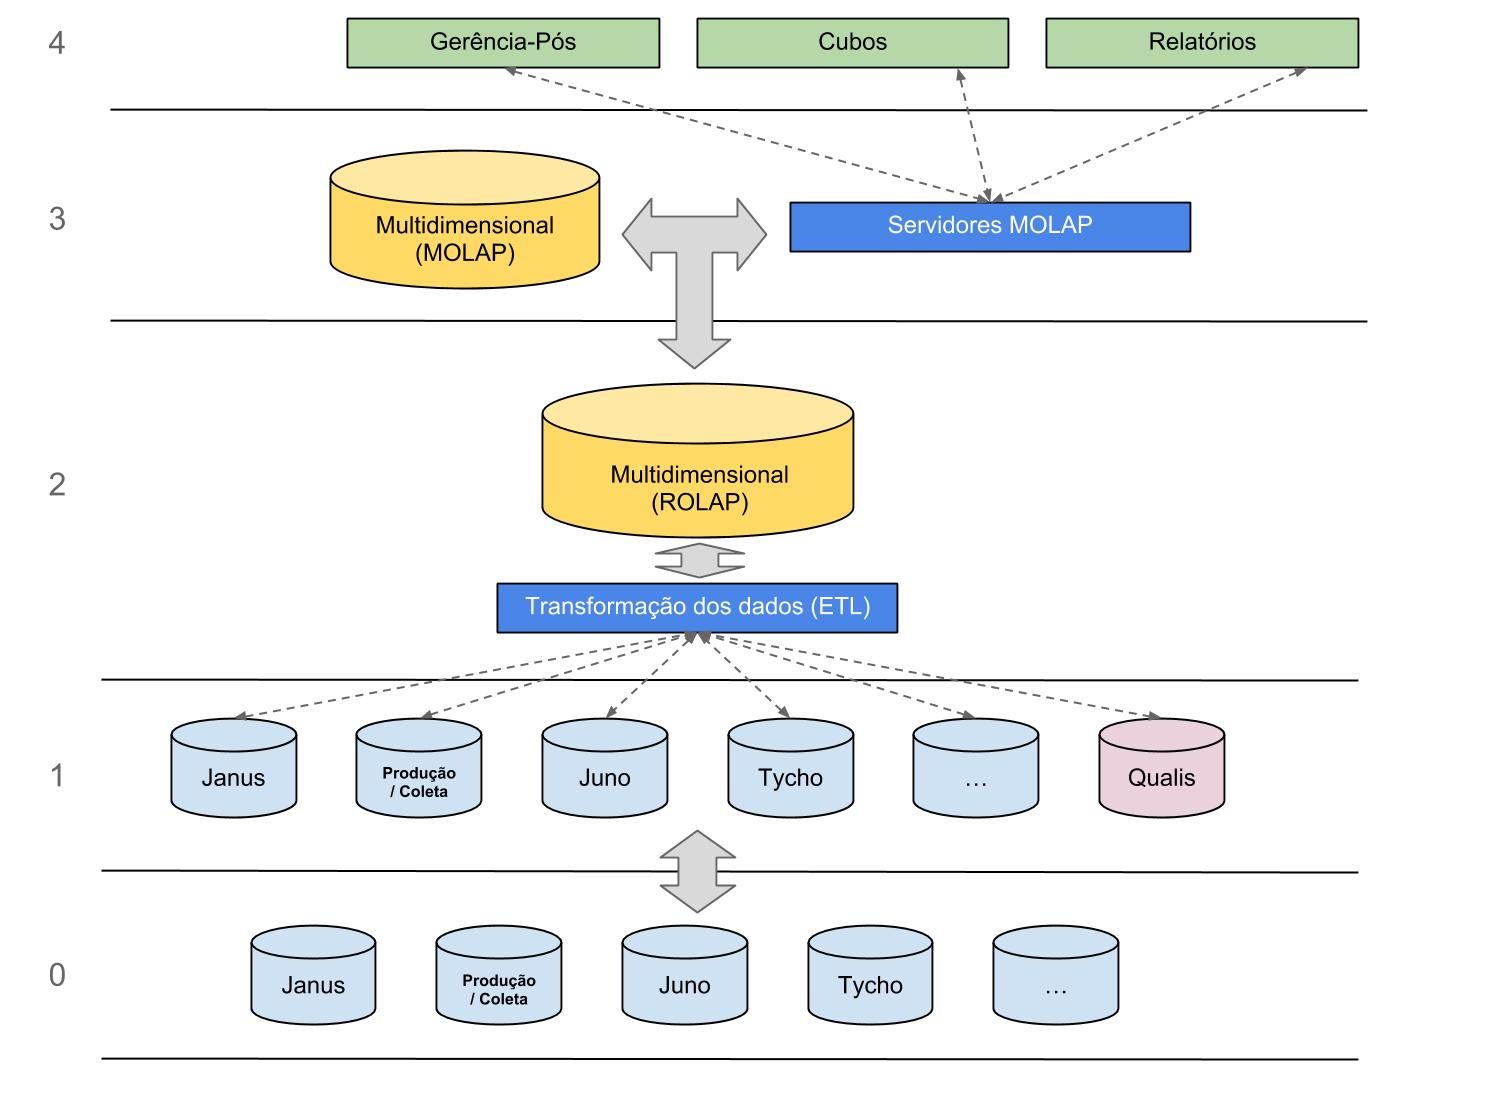
\includegraphics[width=\textwidth]{figuras/arquitetura.jpg}}
  \caption{O mundo dos dados no DataUSP-PósGrad}\label{fig:arq}
\end{figure}

\section{Java}
\label{sec:java}

Java\footnote{Java - http://docs.oracle.com/javase/tutorial/java/javaOO/index.html} é uma linguagem de programação orientada a objetos~\cite{plai_obj} muito popular, usada e aceita comercialmente. Originalmente desenvolvida pela \emph{Sun Microsystems}, em meados de 1995, hoje é mantida pela \emph{Oracle}\footnote{História da tecnologia Java - http://www.oracle.com/technetwork/java/javase/overview/javahistory-index-198355.html}. 
\par
Mais do que uma linguagem, Java é uma plataforma de desenvolvimento composta de bibliotecas pré-compiladas (APIs) e também pela máquina virtual java (JVM). Um programa de computador escrito em Java é compilado em um código específico para ser interpretado pela JVM e, sendo assim, qualquer dispositivo capaz executá-la, independentemente da plataforma utilizada (por exemplo o microsoft windows, linux, mac, android, etc ..), pode executar código Java.
\par
As unidades fundamentais de um programa Java são os Objetos, que são porções de código auto contidos com características similares e com um objetivo em comum. Podem ser usados para descrever objetos abstratos, como um objeto matemático, ou um objeto do mundo real, como por exemplo um carro com seus atributos (cor, modelo, potencia, etc) e também suas funcionalidades (ligar, andar, abrir portas, etc).
\par
Os Objetos em Java são instâncias de uma Classe, um protótipo do Objeto contendo sua descrição por meio de Atributos e Métodos. Os Atributos são os parâmetros e estruturas de dados da Classe, enquanto que os Métodos são as funções da classe, utilizadas para realizar as tarefas pertinentes ao respectivo objeto instanciado.
\par
Valendo-se do conceito de encapsulamento~\cite{plai_obj}, existem Métodos especiais para manipular os atributos de uma Classe Java: os Métodos \emph{getters}, utilizados para obter o valor de um atributo; os Métodos \emph{setters}, para atribuir um valor ao atributo.
\par
Toda Classe contém um Método especial chamado de Construtor Primário. Podendo receber parâmetros externos, instancia um Objeto a partir dessa Classe fazendo as inicializações necessárias. 
\par
Existe ainda um conceito de Classe em Java chamada de Bean. Essa Classe contém apenas Atributos e Métodos \emph{getters} e Métodos \emph{setters}. É usada geralmente para agrupar um conjunto de objetos, como por exemplo os dados cadastrais de um cliente com nome, cpf, data de nascimento e etc. Seu construtor primário não recebe argumentos (em geral não executa ação alguma além de instanciar o Objeto), e assim sua inicialização fica a cargo de quem a instancia.
\par
Uma outra funcionalidade de Java, que é muito usada no projeto DataUSP-PósGrad, é o conceito de Anotações. As Anotações são meta dados adicionados às Classes, Atributos e Métodos com a finalidade de indicar funcionalidades extras. Não alteram o comportamento do código e servem apenas como referência. São usadas no DataUSP-PósGrad para mapear os serviços e seus recursos em seus respectivos endereços de rede.

\section{Jersey}
\label{sec:jersey}
Os RESTful Web Services em java foram apresentados na JSR-311. Uma JSR\footnote{ JSR - \texttt{http://jcp.org/aboutJava/communityprocess/final/jsr311/}} (Java Specification Request) é uma solicitação formal para se incluir novas especificações na plataforma Java.
\par
Como produto final da JSR-311 nasceu a  JAX-RS, uma api\footnote{Application Programming Interface - é uma especificação de como um conjunto de recursos deve ser utilizado, incluindo protocolos, modelo de dados regras de negócio e etc} baseada em anotações para implementar RESTful Web Services em Java. Porém a JAX-RS é apenas uma especificação e sua implementação de 
referência fica a cargo do framework  Jersey.\footnote{Jersey - \texttt{https://jersey.java.net/}}
\par
O Jersey é responsável por intermediar uma requisição HTTP e instanciar a respectiva classe Java que representa o recurso solicitado, por meio do uso de anotações.~\ref{sec:java}

\section{HTTP}
\label{sec:http}
  O HTTP\footnote{HTTP 1.1 - \texttt{http://tools.ietf.org/html/rfc2616}} 
(Hyper Text Transfer Protocol) é um protocolo de comunicação em redes redes de computadores,  
fundamentado no  modelo requisição resposta, utilizado na transferência de hipermídia\footnote{Hipermídia é uma extensão do hipertexto, onde os blocos de informação interconectados por meio de \emph{links} podem ser, além de textos, imagens, sons, vídeos, arquivos, etc.} entre aplicações. É o principal protocolo de comunicação da internet. Seu uso mais comum é a interação de um navegador de internet(cliente) com um servidor web.
\par 
O HTTP implementa oito métodos de requisição que definem a semântica da 
troca de mensagens, ou seja, informam ao servidor a operação a ser realizada ao receber uma requisição do cliente. São eles: GET; POST; PUT; DELETE; HEAD; CONNECT; TRACE; OPTIONS.
\par
Os servidores que implementam o HTTP devem obrigatoriamente implementar dois de seus métodos: HEAD e GET. Além desses, geralmente, são implementados o POST, o PUT e o DELETE. Semanticamente suas funções são:

\begin{itemize}
\item GET - Cujo objetivo é pedir dados ao servidor;
\item POST - Usado principalmente para enviar dados ao servidor (formulários, arquivos, ...);
\item PUT - Também usado para enviar dados, mas com o intuito de modificar uma entrada já existente;
\item DELETE - Para fazer uma requisição de remoção de algum dado.
\end{itemize}
 
Um servidor web pode também receber dados via método GET, porém de modo não seguro uma vez que os dados são enviados explicitamente, concatenados com o endereço da requisição. A ocorrência do símbolo "?" no endereço indica que daí em diante são dados, no formato \emph{parâmetro=valor}, separados pelo símbolo "\&". Exemplo:
\begin{center}
\emph{http://www.webmail.com.br/?username=usuario\&password=senha}
\end{center}

Toda resposta a uma requisição HTTP contém um código numérico de três dígitos. O servidor utiliza esse código para informar ao cliente sobre o estado da requisição. São eles:

\begin{itemize}
\item 1xx - São os códigos para um resposta provisória, apenas informativa. Por exemplo o código 100 indica que o cliente pode prosseguir com a conexão;
\item 2xx - Indicam que a requisição foi recebida, entendida e aceita pelo servidor. O mais famoso exemplo é o código 200, que indica que a requisição foi processada com sucesso;
\item 3xx - São utilizados para redirecionar uma requisição a um outro servidor, por exemplo em balanceamento de carga entre múltiplos servidores de um mesmo serviço;
\item 4xx - Códigos de erros por parte do cliente. O código 404 informa ao cliente que o recurso solicitado não foi encontrado no servidor;
\item 5xx - Códigos de erros por parte do servidor. O código 500 indica que o servidor não pôde atender à solicitação de um recurso por um erro interno.
\end{itemize}

\section{Web Services}

  De acordo com a definição do W3C\footnote{Web Services Architecture - http://www.w3.org/TR/ws-arch/\#whatis} (órgão responsável por regulamentar e sugerir novos padrões para a web), um Serviço Web é uma aplicação projetada para interagir com outras aplicações em redes de computadores, ou seja, um Serviço Web disponibiliza seus recursos mapeados em endereços de rede por meio de uma interface de acesso. Esse acesso ao serviço é feito tipicamente utilizando-se mensagens SOAP , transportadas por meio do protocolo de rede HTTP em formato de um documento XML serializado.

\par
Existem duas arquiteturas principais de Serviços Web, classificados de acordo com a sua interface de acesso: SimpleObject Access Protocol (SOAP) e RepresentationalStateTransfer (REST). O SOAP é um padrão mais antigo e amplamente adotado por empresas e na indústria, enquanto que o REST é uma arquitetura proposta mais recentemente para simplificar o acesso e a implementação de Serviços Web.

\par
Os Serviços Web que implementam a arquitetura REST são denominados RESTFul Web Services.

\section{SOAP}
\label{sec:soap}

O padrão SOAP foi inicialmente concebido para facilitar a comunicação em aplicações protegidas por firewalls. É um protocolo bem definido, atualmente mantido pela W3C\footnote{SOAP specification - http://www.w3.org/TR/soap/}, baseado na troca de mensagens em formato XML. A troca de mensagens pode ser implementada utilizando-se qualquer protocolo de transporte, como por exemplo HTTP, SMTP ou ainda diretamente via TCP ou UDP, cujo propósito é transmitir a mensagem XML serializada.

\par
Uma mensagem SOAP é um documento XML com a seguinte estrutura:

\begin{figure}[H]\centering
  \centerline{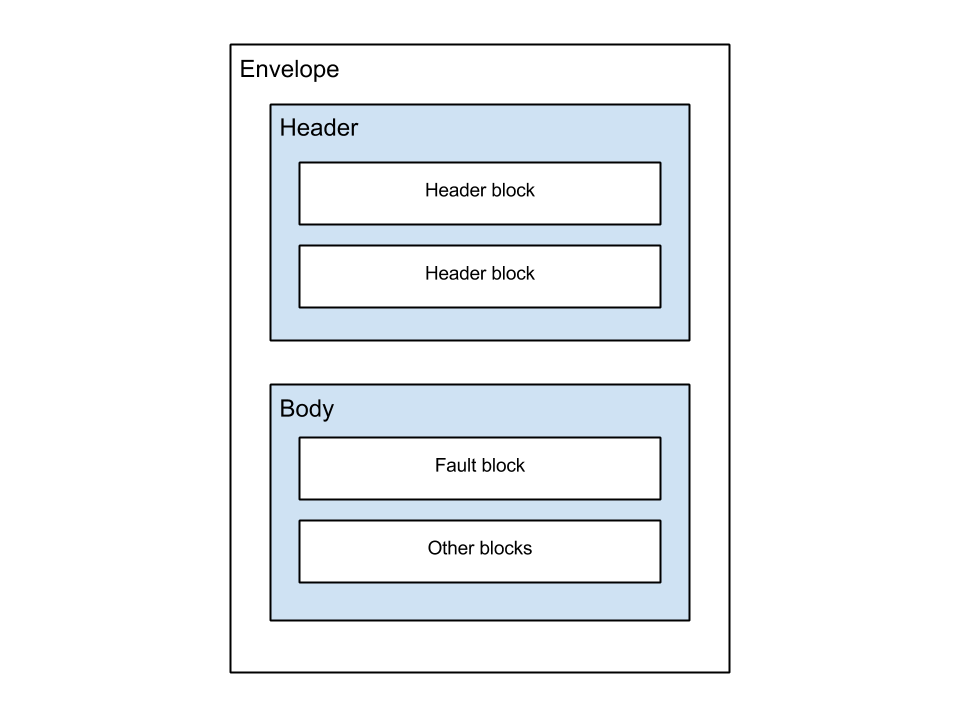
\includegraphics[width=\textwidth]{figuras/soap.png}}
  \caption{Diagrama de uma mensagem SOAP}\label{fig:soap}
\end{figure}

Onde:
\begin{itemize}
\item<Envelope> é o elemento principal e contém outros 2 elementos, o <Header> e o <Body>;
\item<Header> é opcional e quando presente precisa ser o primeiro descendente do <Envelope>. Contém informações específicas que serão processadas por nós intermediários, antes da mensagem atingir o destinatário final; 
\item<Body> sessão destinada à requisição de um recurso ao Serviço Web. Contém o endereço especifico do recurso solicitado, nome e os dados;
\item<Fault> subelemento  do <body> destinado a mensagens de erro.
\end{itemize}

\section{REST}
\label{sec:rest}

O REST , mais recentemente proposto~\cite{RTF}, não é exatamente um protocolo mas sim uma arquitetura proposta para simplificar o acesso e a implementação de Serviços Web. 
\par
Não há um modelo padrão para uma mensagem REST, podendo-se utilizar diversos tipos de documentos ou formatos de dados, incluindo o próprio XML ou texto plano. Isso permite adequar o modelo de dados adotado na requisição de cada recurso fornecido pelo Serviço Web.
\par
 A troca de mensagens, assim como o acesso aos recursos de um Serviço Web REST, são realizados utilizando-se exclusivamente o protocolo HTTP , por meio de seus métodos nativos, como por exemplo GET, POST, DELETE, e etc. Os recursos disponibilizados são identificados por meio de endereços únicos de rede (URI), e não no interior da mensagem como no caso do SOAP.
\par
 Um Serviço Web REST não mantém o estado de dados (contexto) entre requisições, ou seja, cada requisição por um recurso do Serviço Web contém todos os dados necessários para a solicitação na mensagem.


\subsection{REST vs SOAP}

As principais diferenças entre REST e SOAP estão no tipo de mensagem utilizada na comunicação, e no modo como essas mensagens são transportadas.
\par
Uma mensagem SOAP tem um formato especifico e bem definido, denominado envelope SOAP. Os dados enviados a um Serviço Web SOAP precisam necessariamente estar contidos nesse envelope que, além dos dados, contém outras informações relevantes para se obter acesso a um recurso, como seu nome, seus parâmetros, seu endereço específico dentre outras informações. 
\par
 Já uma mensagem REST não possui um formato de dados específico pré-definido, no qual qualquer tipo de hipertexto pode ser usado, por exemplo texto plano, o próprio XML, JSON e inúmeros outros. Em um mesmo Serviço Web pode haver recursos que utilizam mensagens de tipos distintos, aumentando a flexibilidade e melhor adequando o modelo de dados ao tipo de aplicação. Além disso, ao utilizar-se o formato JSON\footnote{JSON, Java Script Object Notation - http://www.json.org/}, por exemplo, ao invés do XML, uma mesma mensagem pode ficar muito mais compacta , diminuindo o fluxo de dados na rede, e mais simples de interpretar por quem solicita tal recurso.
\par
Quanto ao modo de transporte de mensagens, o SOAP teoricamente pode utilizar qualquer protocolo de transporte de rede, porém na prática o mais utilizado é o HTTP, assim como o REST. A diferença é que apesar de ambos empregarem o HTTP, o SOAP o utiliza apenas como protocolo de transporte, enquanto que o REST o utiliza também para controle.
\par 
 Os recursos de um Serviço Web RESTful são acessados por meio dos métodos de controle do HTTP~\ref{sec:http}, juntamente com um endereço único que identifica cada recurso fornecido pelo Serviço Web. Já em um Serviço Web SOAP o método HTTP utilizado na requisição de um recurso geralmente é ignorado, ficando a cargo do serviço fazer o controle da transação de acordo com o recurso solicitado descrito no envelope SOAP. Por exemplo, haverá um recurso getDados() para retornar alguma informação, e um outro recurso sendDados() para receber dados, no qual o Serviço Web terá a competência de resolver a requisição.
\par
 Utilizar diretamente os métodos do HTTP, que já é também responsável por transportar os dados na rede, tem a vantagem de simplificar a implementação da interface de acesso aos recursos de um Serviço Web, aumentando assim sua escalabilidade, que além de mantê-la mais homogênea ainda facilita o consumo dos recursos pelos usuários do serviço.
\par As figuras~\ref{fig:rest_msg} e~\ref{fig:soap_msg} ilustram, respectivamente, as mensagens de requisição e resposta de um mesmo recurso em um Serviço Web REST, e de sua variante SOAP:
\\\\\\\\\\\\
 
\begin{figure}[H] 
\begin{Verbatim}[frame=single,fontsize=\footnotesize,framesep=3mm,label=requisição,numbers=left,numbersep=1mm]
http://nhagaexemplo.usp.br/servicos/almoco/central

GET servicos/almoco/central HTTP/1.1
Accept: application/json, text/javascript, */*;
Content-Length: nnn

\end{Verbatim}
\begin{Verbatim}[frame=single,fontsize=\footnotesize,framesep=3mm,label=resposta,numbers=left,numbersep=1mm]
HTTP/1.1 200 OK
Content-Type: application/json

{"Mistura":"Carne Moida","Guarnicao":"Batata Gratinada",
 "Sobremesa":"Melancia","Suco":"Uva",
 "Base1":"Arroz","Base2":"Feijão"}
\end{Verbatim}
\caption{Requisição e resposta de um recurso de um Serviço Web REST}
\label{fig:rest_msg}
\end{figure}

\begin{figure}[H]
\begin{Verbatim}[frame=single,fontsize=\footnotesize,framesep=3mm,label=requisição,numbers=left,numbersep=1mm]
POST /Cardapio HTTP/1.1
Host: www.nhagaexemplo.usp.br
Content-Type: application/soap+xml; charset=utf-8
Content-Length: nnn

<?xml version="1.0"?>
<soap:Envelope
xmlns:soap="http://www.w3.org/2001/12/soap-envelope"
soap:encodingStyle="http://www.w3.org/2001/12/soap-encoding">

<soap:Header>
    <m:dateAndTime>2013-09-29T13:20:00.000-05:00</m:dateAndTime>
</soap:Header>

<soap:Body xmlns:m="http://www.nhagaexemplo.usp.br/cardapio">
    <m:GetAlmoco>
        <m:Restaurante>Central</m:Restaurante>
    </m:GetAlmoco>
</soap:Body>

</soap:Envelope>
\end{Verbatim}

\begin{Verbatim}[frame=single,fontsize=\scriptsize,framesep=3mm,label=resposta,numbers=left,numbersep=1mm]
HTTP/1.1 200 OK
Content-Type: application/soap+xml; charset=utf-8
Content-Length: nnn

<?xml version="1.0"?>
<soap:Envelope
xmlns:soap="http://www.w3.org/2001/12/soap-envelope"
soap:encodingStyle="http://www.w3.org/2001/12/soap-encoding">

<soap:Header>
    <m:status>1</m:status>
    <m:restaurante>central</m:restaurante>
</soap:Header>

<soap:Body xmlns:m="http://www.example.org/stock">
    <m:GetAlmocoResponse>
        <m:Mistura>Carne Moida</m:Mistura>
	    <m:Guarnicao>Batata Gratinada</m:Guarnicao>
	    <m:Sobremesa>Melancia</m:Sobremesa>
	    <m:Suco>Uva</m:Suco>
	    <m:Base1>Arroz</m:Base1>
	    <m:Base2>Feijão</m:Base2>
    </m:GetAlmocoResponse>
</soap:Body>

</soap:Envelope>
\end{Verbatim}
\caption{Requisição e resposta de um recurso de um Serviço Web SOAP}
\label{fig:soap_msg}
\end{figure}

\subsection{RESTFul web services}
\label{sub:restful}
A popularidade dos Serviços Web RESTful tem aumentado devido, principalmente, a maior simplicidade de acesso aos seus recursos, uma vez que as requisições são realizadas por meio dos métodos nativos do protocolo HTTP , que também é utilizado como protocolo de transporte de dados. Além disso, a não obrigatoriedade de utilizar-se mensagens XML para a troca de informações, permite o uso de modelos de dados mais simples, como por exemplo o JSON, o que diminui a sobrecarga de dados (metadados) na rede.
\par
Os Serviços Web são amplamente utilizados na Internet, por esse motivo o desempenho de tais aplicações é um fator muito importante. Conforme o trabalho apresentado por Snehal Mumbaikar e Puja Padiya~\cite{SMPP}, um Serviço Web RESTFul é uma melhor alternativa para implementação de aplicações na Web, pois reduz a quantidade de dados na rede, melhorando o tráfego de informação útil. Além do mais reduz a latência de acesso com mensagem mais compactas em tamanho de bytes. Os Serviços Web RESTful são mais leves e fáceis de implementar que os Serviços Web SOAP pois são auto descritivos com maior flexibilidade e menor sobrecarga.  Como o objetivo do Sistema DataUSP-PosGrad é o de gerar relatórios de modo eficiente e rápido com o mínimo de impacto no tráfego de dados na rede, além de permitir seu uso por outros sistemas corporativos da USP e viabilizar seu acesso por dispositivos móveis, como tablets e smartfone, foi adotada a arquitetura REST para sua implementação e projeto. 

\section{SQL}
\label{sec:sql}

SQL ou Structured Query Language (~\cite{navat},cp.4) é uma linguagem declarativa usada para acessar os dados de um SGBD\footnote{SGBD - Sistema Gerenciador de Banco de Dados} relacional. Suas cláusulas podem ser divididas em duas categorias: a DDL e a DML.
\par A DML (Data Manipulation Language) é usada para fazer consultas, modificar e inserir dados no banco. As principais cláusulas são o SELECT, INSERT, UPDATE e DELETE. Exemplo:

\begin{figure}[H]
\begin{minted}[frame=single,linenos,mathescape,fontsize=\small]{sql}
SELECT <coluna1,coluna2,...> FROM <tabela> 
       WHERE <condicao1 AND condicao2 ...>
       
INSERT INTO <tabela> (coluna1,coluna2,...) 
       VALUES (valor1,valor2,...)     
       
UPDATE <tabela> 
SET <coluna1>=<valor1>, <coluna2>=<valor2>, ... 
WHERE <condicao>

DELETE FROM <tabela> WHERE <condicao>
\end{minted}
\caption{Exemplos de consultas SQL}
\label{lst:ia}
\end{figure}

\par A DDL (Data Definition Language) descreve e modifica a estrutura das tabelas e de outros objetos do SGBD, como usuários e permissões de acesso. Exemplo:

\begin{figure}[H]
\begin{minted}[frame=single,linenos,mathescape,fontsize=\small]{sql}
CREATE TABLE `Usuarios` (
  `id` int(11) unsigned NOT NULL AUTO_INCREMENT,
  `email` varchar(255) COLLATE utf8_bin NOT NULL,
  `nome` varchar(255) COLLATE utf8_bin NOT NULL,
  `instituicao` varchar(255) COLLATE utf8_bin NOT NULL,
  `cargo` varchar(255) COLLATE utf8_bin NOT NULL,
  `associacao_id` int(11) NOT NULL,
  `modified` datetime NOT NULL,
  PRIMARY KEY (`id`),
  FOREIGN KEY (associacao_id) REFERENCES Associacoes(id)
) ENGINE=InnoDB AUTO_INCREMENT=1 DEFAULT 
  CHARSET=utf8 COLLATE=utf8_bin;
\end{minted}
\caption{Exemplo de criação de tabela em SQL}
\label{lst:sql_ddl}
\end{figure} 

\section{JavaScript}
Javascript é a linguagem de script mais popular da web, presente na maioria das paginas HTML atuais. Tem tipagem fraca , type-safety ~\cite{plai} e é capaz de representar múltiplos paradigmas como orientação a objetos, funcional e imperativo. Foi formalizada no padrão ECMA-262.\footnote{ECMA-262 - \texttt{http://www.ecma-international.org/ecma-262/5.1/}}
\par
É uma linguagem amplamente usada para processar dados do lado cliente de uma aplicação web, por exemplo:
\begin{itemize}
\item  modificando a página dinamicamente e interagindo com o usuário;
\item  tratando os dados recebidos da página antes de enviar ao servidor;
\item  fazendo chamadas assíncronas ao servidor sem recarregar a página.
\end{itemize}


\subsection{JQuery}
\label{sub:jq}
Jquery\footnote{JQuery - \texttt{http://jquery.com/}} é uma biblioteca de JavaScript que facilita e simplifica a manipulação de documentos HTML e o tratamento de eventos. Por exemplo, o trecho de código abaixo troca a cor de todos os links em uma página, utilizando JQuery e JavaScript puro respectivamente:

\begin{minted}[frame=single,linenos,mathescape,label=Jquery]{js}
\$("a").css('color','red');
\end{minted}

\begin{minted}[frame=single,linenos,mathescape,label=javaScript]{js}
var l = document.getElementsByTagName("a");
for(var i=0; i < l.length; i++){
  l[i].style.color = "red";
}

\end{minted}

O seletor \$() em JQuery utiliza a mesma sintaxe da notação de estilos css\footnote{CSS - http://www.w3.org/TR/CSS21/cover.html\#minitoc} para selecionar um elemento.Exemplo:

\begin{itemize}
\item \emph{\$("\#id")} para selecionar um id;
\item \emph{\$(".cl")} para selecionar elementos que possuem a classe "cl";
\item \emph{\$("tag")} para selecionar uma tag qualquer de HTML.
\end{itemize}

Enquanto que em JavaScript puro há um método específico para cada tipo de elemento:
\begin{itemize}
\item  \emph{document.getElementById("id")} para selecionar um id;
\item  \emph{document.getElementsByClassName("cl")} para selecionar um elemento que possui a classe "cl";
\item  \emph{document.getElementsByTagName("tag")} para selecionar uma tag qualquer.
\end{itemize}

Jquery possui ainda diversos plugins para prover funcionalidades úteis, como preencher datas, auto completar campos de busca, mostrar uma sequência de imagens com efeitos de transição, dentre muitas outras. Isso tudo permite escrever um código menor, mais legível e de fácil manutenção.

\subsection{AJAX}
\label{sub:aj}
Ajax~\cite{ajax} (Asynchronous JavaScript and XML) foi um termo cunhado por Jesse Jamers Garret para designar um conjunto de tecnologias para fazer requisições assíncronas a um Serviço Web, isto é, adicionar ou modificar dados em uma página web(site) dinamicamente, sem a necessidade de recarregá-la completamente. Esse tipo de requisição é feita usando-se JavaScript, ou por meio de JQuery. Apesar do nome é possível usar JSON como formato de dados ao invés de XML.
\par
Uma requisição Ajax por intermédio de JQuery tem o seguinte formato:

\begin{minted}[frame=single,linenos,mathescape]{js}
\$.ajax({
    url : "/datausppg/recursos/listagem",
    type: "POST",
    data : formData,
    success: function(data, textStatus, jqXHR)
    {
        //data - dados retornados pelo servidor
    },
    error: function (jqXHR, textStatus, errorThrown)
    {
        
    }
});
\end{minted}
Onde:
\begin{itemize}
\item \emph{url}: endereço do recurso solicitado;
\item \emph{type}: tipo de requisição (GET, POST, …);
\item \emph{data}: dados a serem enviados de acordo com o tipo de requisição;
\item \emph{success}: função executada caso o servidor retorne um código HTTP de sucesso ( possivelmente enviando dados );
\item \emph{error}: função executada quando o servidor responde com um código HTTP de erro;
\end{itemize}

\subsection{HTML5}
\label{sub:h5}
HTML (HyperText Markup Language) é a linguagem usada pelos navegadores de internet (Web Browsers) para interpretar os documentos (páginas) da web. Sua estrutura é composta de tags, que são marcadores que identificam os elementos que compõe um documento HTML.

\begin{figure}[H]
\begin{minted}[frame=single,linenos,mathescape]{html}
<!DOCTYPE html>
<html>
    <head>
        <meta charset="UTF-8">
        <title>Titulo do documento</title>
    </head>
    <body>
        <!-- Conteudo do documento -->
    </body>
</html>
\end{minted}
\caption{Estrutura básica de um documento HTML}
\label{lst:html}
\end{figure}

Sua versão mais recente é o HTML5 \footnote{ HTML - \texttt{http://www.w3.org/community/webed/wiki/HTML}}, cujo um dos  propósitos é diminuir a dependência de plugins externos e scripts (com o advento de novas tags para renderização de áudio, video e animações ). Além disso, passa a suportar novas funcionalidades que visam melhorar a padronização do código, assim como sua portabilidade entre diferentes plataformas e navegadores.

\subsection{Gráficos - FusionCharts}
\label{sub:fc}

Fusion Charts\footnote{ Fusion Charts - \texttt{http://www.fusioncharts.com/}} é uma biblioteca javaScript para construir gráficos. Usada conjuntamente com HTML5, os gráficos são renderizados unicamente por meio de javaScript, criando modelos animados em três dimensões sem a necessidade de se utilizar algum plugin externo (como o Adobe Flashplayer por exemplo ), reduzindo a carga no servidor e melhorando o desempenho do lado cliente. A figura~\ref{fig:fusion} ilustra alguns modelos de gŕaficos construidos com o Fusion Charts.

\begin{figure}[H]
    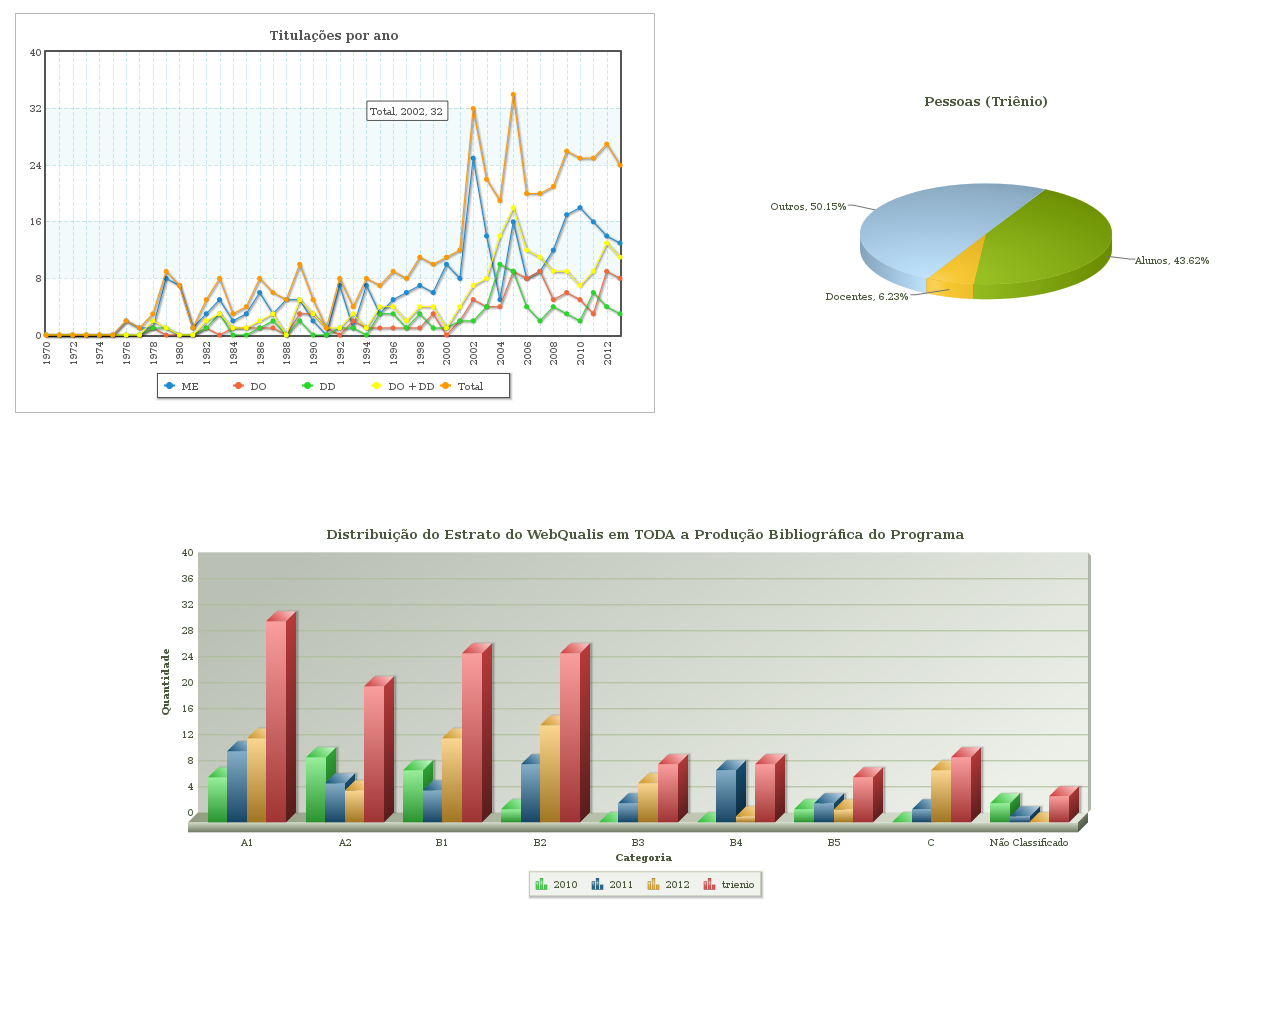
\includegraphics[width=\textwidth]{figuras/graf_ex}
    \caption{Alguns modelos de gráficos disponíveis no Fusion Charts}
    \label{fig:fusion}
\end{figure}

\section{Web Crawler}
\label{sec:wc}
  Web Crawler~\cite{craw} é um programa de computador que navega na internet de modo autônomo, visitando páginas e lendo seu conteúdo, geralmente com a finalidade de indexação.
  \par
  Duas das principais ferramentas para interagir com a web em linux são o curl e o wget. Enquanto que o wget é apenas um comando o curl usa a biblioteca libcurl\footnote{libcurl - \texttt{http://curl.haxx.se/libcurl/}}, disponível em múltiplas plataformas e suportada por diversas linguagens de script, dentre elas Python.
  \par
  A biblioteca libcurl trabalha com diversos protocolos incluindo o HTTP, permitindo simular o comportamento de um navegador de internet, inclusive utilizando cookies\footnote{HTTP Cookie - É um arquivo de texto salvo pelo navegador do lado cliente usado pelo servidor para obter dados anteriores da navegação de seus usuários}, enviando dados de formulários, fazendo autenticação e etc. Além disso pode-se configurar o cabeçalho de uma requisição para incluir dados adicionais e até mesmo se passar por algum navegador específico, como o Mozilla Firefox por exemplo (Algumas páginas fazem redirecionamentos específicos e até mesmo bloqueiam conteúdo dependendo do navegador usado).
  \par
  Por meio da bibliotea libcurl é possível construir uma aplicação que navegue na internet, extraindo dados de páginas específicas afim de utlilizá-los como uma fonte externa de informações, armazenando-os em um banco de dados.
  
\subsection{Python}

Python\footnote{Python - \texttt{http://www.python.org/}} é uma linguagem de programação interpretada que vem ganhando notoriedade por sua versatilidade e facilidade de usar. É uma linguagem multiparadigma com uma variedade extensa de bibliotecas para as mais diversas aplicações ( por exemplo o framework mvc django\footnote{Django - \texttt{https://www.djangoproject.com/}} e a biblioteca de ferramentas científicas SciPy\footnote{SciPy - \texttt{http://www.scipy.org/}} ).
\par
Utilizando as bibliotecas pycurl e pyquery é fácil construir um script para navegar na internet. A primeira é a implementação em python da libcurl e a segunda permite percorrer um documento HTML de modo similar ao JQuery.


\section{Pentaho}
\label{sec:pentaho}
Pentaho Business Analytics\footnote{Pentaho - \texttt{http://sourceforge.net/projects/pentaho/}} é um conjunto de ferramentas de BI (Business Inteligence) para fazer análise, visualização e transformação de dados por meio de interfaces amigáveis e intuitivas. O pacote tem licença GPL, ou seja é open source, apesar de possuir também uma versão comercial.
\par
Uma das ferramentas do Pentaho é o Kettle, utilizada para fazer acesso e transformação de dados (ETL~\cite{VR}) entre diferentes fontes, que vão desde arquivos de texto às mais diversas bases de dados. Muito utilizada na construção e manutenção de um Data Warehouse. 

\begin{figure}[H]
    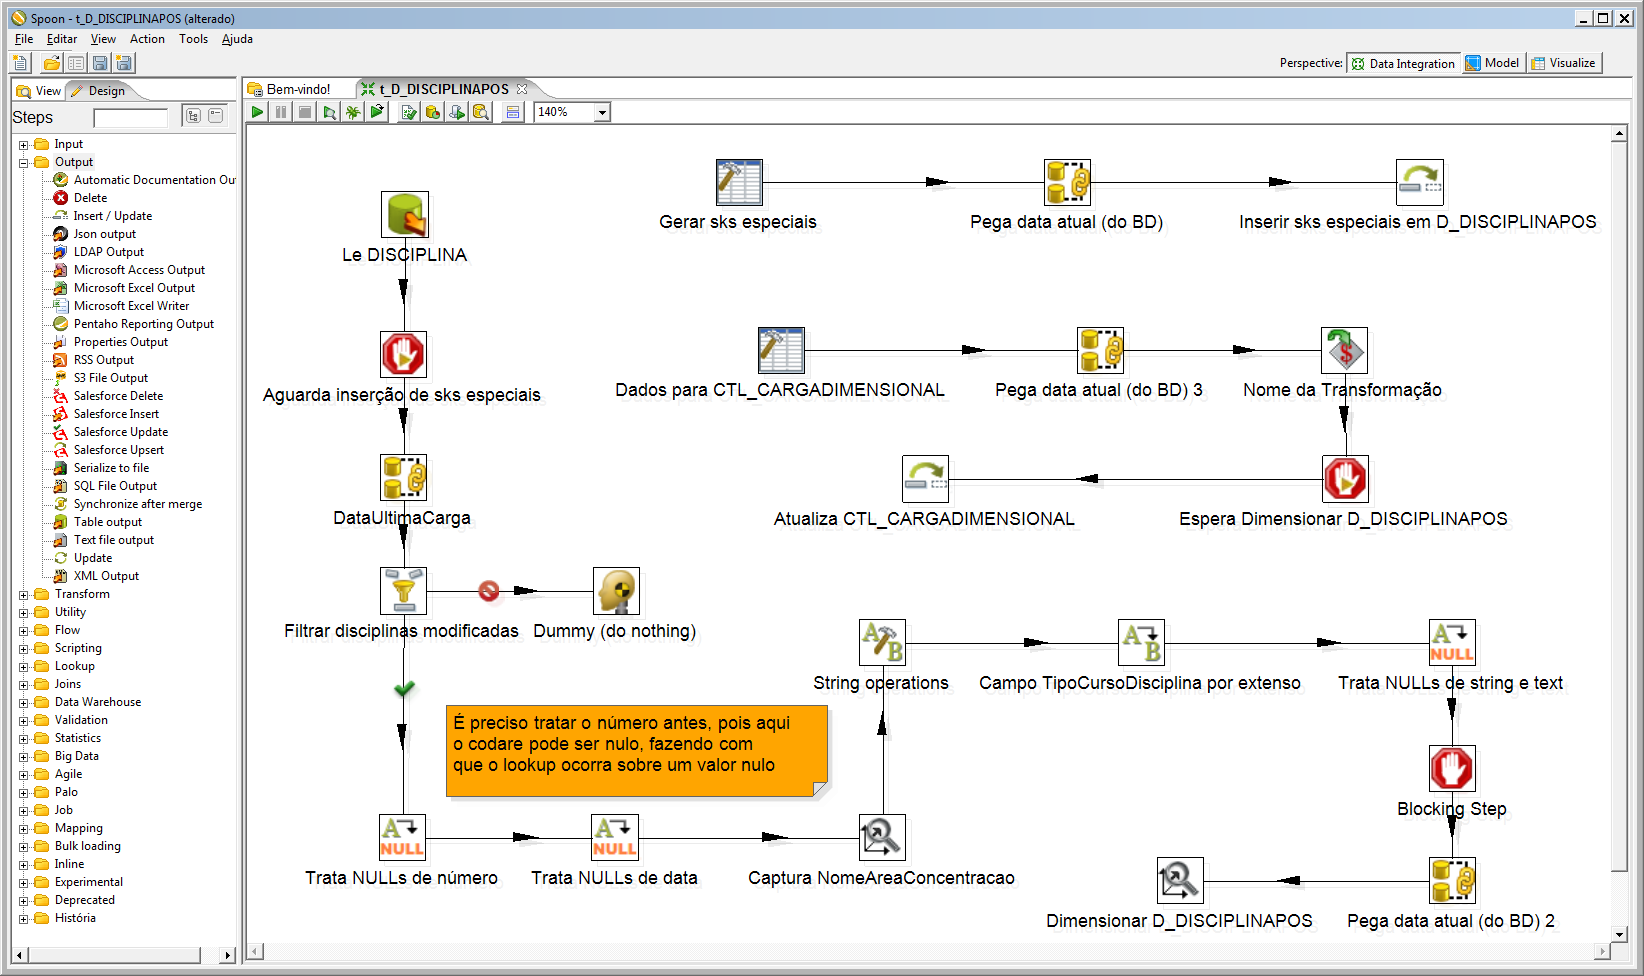
\includegraphics[width=\textwidth]{figuras/pentaho.png}
    \caption{Ferramenta Kettle do pacote Pentaho}
    \label{fig:kettle}
\end{figure}

